\documentclass{article}
\usepackage{graphicx} % Required for inserting images
\usepackage{natbib}
\usepackage{amsmath}
\usepackage{comment}
\usepackage{url} 
\usepackage[hidelinks]{hyperref}
\usepackage[T1]{fontenc}
\usepackage{mathpazo,euler}
\usepackage[scaled=0.9]{DejaVuSans}
\usepackage[utf8]{inputenc}
\usepackage{listings}
\usepackage{tabularx}
\usepackage{amsfonts}
\usepackage{booktabs}
\usepackage{siunitx}
\usepackage{geometry}

\geometry{margin=1.5in}
\lstset{basicstyle=\ttfamily}
%\documentclass[11pt]{article}
\setlength{\parskip}{1em} % 1em is an example value; adjust as needed
\bibliographystyle{abbrvnat}
\setcitestyle{authoryear,open={(},close={)}} % Citation-related commands

%\title{First Year Paper}
\title{First Year Paper} % Add your subtitle here
% title ideas
% Genetic architecture implication on rapid evolutionary dynamics & detectability of causal loci after a rapid evolution event  



%\subtitle(Advisor: Moisés Expósito Alonso)
\author{Tatiana Bellagio \\ Advisor: Moisés Expósito Alonso}
\date{November 2023}

\let\oldparagraph\paragraph
\renewcommand{\paragraph}[1]{\oldparagraph{#1}\mbox{}\\}

\begin{document}

\maketitle

\begin{abstract}
In the face of anthropogenic climate and land use crises, environments are changing faster than ever and species must adapt to keep up and avoid extinction. While this has motivated much theoretical and simulation-based research to study the role of genetic architecture in rapid environmental adaptation, these studies are rarely parameterized with realistic setups let alone validated through feasible experiments. Here, I use population genetic simulations varying genetic architecture parameters, from monogenic to polygenic, from low heritable to high heritable traits, in experimental setups that closely match Evolve \& esequence experiments with \textit{Arabidopsis thaliana} . These include realistic population sizes, survival and fecundity distributions, partial selfing, strengths of selection, and starting genetic material through starting simulations with whole-genome variant data. I then investigate the effect of such parameters and the outcome of population adaptation or extinction, and benchmarked the detectability of adaptive loci across genetic architecture after rapid adaptation. My results indicate that traits with higher polygenicity significantly enhance survival probabilities in rapidly changing environments, while the influence of heritability varies depending on genetic architecture complexity. Finally this research highlights the lack of methodologies to accurately detect adaptive loci across environments in experimental evolution approaches. 
\end{abstract}

\tableofcontents
\newpage % Starts a new page after the table of contents

\section{Introduction}
\subsection{Shift, Adapt or Perish}
When species face environmental changes that displace them from their ecological niche, there are only three possible outcomes: shift their geographical distribution to track suitable environments, adapt to the newly imposed conditions, or face local to global extinction. Adaptation is the process by which a population becomes better suited to the new environment through natural selection acting over the population's standing and de novo genetic variation. In the face of rapid anthropogenic  environmental changes (IPCC 2022) , adaptation through evolution must also be rapid to ensure persistence of populations and avoid extinction. Thus, specifically understanding rapid eco-evolutionary dynamics has become of utmost importance \citep{Waldvogel2020-dh, Palumbi2002-li, Stockwell2003-da}. 

\subsection{But what is rapid evolution?}
Evolution has been historically thought of as a slow and gradual process occurring over extensive timescales, often spanning thousands to millions of years. However, genetically based rapid phenotypic changes have been shown to be pervasive in nature, such as the famous peppered moth \citep{Cook2013-bs}, insecticide resistance in \textit{Drosophila} \citep{Daborn2002-is},  beak size in Darwin’s finches \citep{Grant2008-uc}, \textit{Brassica  rapa} flowering time in response to climate fluctuations, and the evolved resistance to agricultural products in 200 plant species (Weedscience.org, 1993). 

Rapid evolution, can be defined based on the short number of generations in which a genetic change occurs, but also as the convergence of ecological and evolutionary times \citep{Hairston2005-qo}. This highlights the importance of rapid evolution as one of the more applied domains within evolutionary biology. Coupled with advances in genome sequencing technology that have led to an increase in the genomic data on non-model organisms, the understanding of eco-evolutionary dynamics have the potential to address urgent conservation issues. Understanding and predicting the pace and direction of evolutionary changes can inform conservation strategies and management practices. (Hoffmann  et al. 2015; Coulson et al. 2017; Bay et al. 2017a).

As highlighted in \citep{Yamamichi2022-yj} short-term eco-evolutionary dynamics, despite their inherent interdisciplinary nature, have been mostly studied solely from an ecological perspective and tend to focus on adaptation at the phenotypic level without considering the genetic part of the evolutionary process. More studies are needed in the evolutionary aspect of rapid adaptation to understand intertwined processes and to make more accurate predictions. \citep{Rudman2022-uc}

\subsection{Trait architecture and adaptation}

Discussions concerning  how and where adaptive loci are distribute across the genome have come a long way. Since Darwin (Darwin 1859) and Huxley (Huxley 1860) there has been debates about whether the nature of adaptation is characterized by incremental, subtle variations in many loci or by abrupt changes on only a few of them. These are foundational unsolved questions in evolutionary biology, with compelling evidence showing that both cases can be true, and that there is considerable heterogeneity in architectures among adaptive traits \citep{Orr1992-xj, Orr1998-pr}, let alone complexities not discussed hereincluding  the effect of structural variation, epistasis, pleiotropy, and ploidy. 

The implications of genetic architecture on population dynamics have been widely documented. For example, genetic architecture acting as a buffer for adaptive alleles through dominance \citep{Yamamichi2017-uj}, or the implication of the number of loci affecting reproductive incompatibility and determining speciation \citep{Orr1996-eq}. Many more are listed in \citep{Bertram2019-sg}. Delving deeper on a more narrow sense definition of genetic architecture--defined as the number, frequency, distribution of effects and penetrance of causal loci-- two qualitative different waves of research can be described. The first, rooted on traditional population genetics, focuses on selective sweeps where adaptation depends only on one or a few adaptive loci (Hermisson and Pennings 2005;  Hermisson and Pennings 2005; Barrett and Schluter 2008). The second, with the advent of newer sequencing technologies and statistical methodologies, that showcase the polygenic nature of most traits (cite). Since then, there has been major interest in the evolutionary dynamics of polygenic adaptation \citep{John2020-xc}  \citep{Jain2017-mb}, \citep{Barghi2020-aa} \citep{Hayward2021-ji, Stetter2018-st, Thornton2019-ww},  \citep{Hollinger2019-lb}. 

However, often these studies focus on the impact of genome architecture in adaptation in general, spanning long time periods and extending over hundreds or thousands of generations and relying on a tremendous amount of \textit{de novo} mutation, rather than studying their impacts in short, rapid adaptation. As shown by \citep{Orr2008-jl}, adaptation to big environmental challenges over short periods can be difficult when relying on new mutations, and populations will often decline to extinction. Instead, rapid adaptation is likely to proceed through standing genetic variation \citep{Barrett2008-tj}. The implication of different trait genetic architectures from standing genetic variation on the dynamics of rapid evolution has been limited to a handful of studies \citep{Gomulkiewicz2010-wr, Kardos2021-jd}, showing conflicting results, and often conducted in highly abstract simulations and theoretical parameter spaces.

\subsection{How can we practically study rapid evolutionary dynamics to the environment? }
Evolutionary adaptation to the environment has often been studied through either time series (longitudinal studies), or through transplantation to different environment (cross-sectional studies). For instance, wild or experimental populations and their genetics can be tracked over time in Evolve and Resequence (E\&R) experiments. Alternatively, signals of adaptation can be studied of populations transplanted in common gardens across environmental gradients. 

On one hand, E\&R \citep{Schlotterer2015-yz}, are a well established methodology in evolutionary biology. They combine the principles of experimental evolution with sequencing techniques, and consist on applying selective pressures in controlled environments to then pool sequence the evolving populations over time. Some successful examples include \citep{Bergland2014-ud, Kapun2021-cd, Rudman2022-uc}. E\&R are particularly well-suited to study rapid evolution because they allow researchers to observe evolutionary changes over relatively short periods. This experimental approach coupled with genomic scans has shown to be powerful to detect genomic regions responsible for populations adaptation \citep{Vlachos2019-nf}. For example \citep{Bergland2014-ud} was able to identify adaptive allele shifting seasonally in \textit{Drosophila} populations. 

On the other hand, one of the most widely used experimental designs to find signals of local adaptation are common gardens \citep{Lee-Yaw2016-td}. Common gardens consist of growing individuals from different origins in the same set of controlled environments. By controlling the environment, any differences observed among populations are likely due to genetic variation. Some successful examples are \citep{Exposito-Alonso2019-hs, Lepais2014-za}. 

A combined approach of E\&R and common garden experiments could be unusually powerful to better understand climate-driven rapid evolutionary dynamics and to identify genomic regions responsible for climate adaptation. With this in mind, a multi-generation and globally distributed common garden experiment was conducted (\url{http://grene-net.org/}). Using over 230 highly diverse founder \textit{Arabidopsis thaliana} lines were mixed, planted and resequenced over 5 years across 32 locations in the Northern hemisphere. Nevertheless, GrENE-net's potential to identify climate adaptation regions hinges on using the right analytical methods, and the ideal tool would need to effectively process and interpret complex genomic data across space and time. 

As it is often the case with innovative approaches, the most powerful tool for its purpose is still in development. In this context, simulations are specially suited to lay a ground truth for expected results, test available methodologies, detect their weaknesses and highlight areas where further development is necessary.  Complex and highly-realistic population genetic simulations are now feasible through SLiM [CITE]. These  give a fast, synthetic and straightforward path to understand the behaviour of key parameters and layout expected evolutionary results for the real world. 





\subsection{Detecting adaptive loci after rapid evolution}

Ultimately, in studies of rapid adaptation we want to identify signals that convincingly point to evolutionary dynamics not explained by genetic drift, and ideally identify the loci and genomic architecture that enabled such adaptive process. Detecting genomic regions responsible for adaption to the imposed conditions in experimental evolution, or to the current environment in natural populations has been one of the biggest goals in evolutionary biology and conservation. This information can be extremely valuable, and can have direct applications, like genetically targeting natural populations at extinction risk. (cite) Nevertheless, detecting loci underlying an adaption process is not a trivial task. Some of the approaches used include: genomic scans of selection based on polymorphism data, Genome Wide Association Studies (GWAS) linking genotypes with putatively adaptive phenotypes, and Genome Environmental Association Studies (GEAS) linking genotypes with different environments or features of the lanscape. Nonetheless it is still not clear if any of them would be particularly suited to detect signals of *rapid* adaptation in E\&R and common garden experiments such as the ongoing GrENE-net experiment.

\subsubsection{Genome scans}
Genome scans are the most widely developed and used methodology in evolutionary biology to detect genomic regions under selection (cites). Their main assumption is that selected regions would show a diversity reduction when compared to the rest of the genome. Depending on the genetic architecture of the adaptive trait,  genomic footprints of selection can be one of three types: hard sweeps, soft sweeps, or polygenic signals. Historically, most selection scans have focused on detecting hard sweep (cite) rooted on a classical population genetics view of adaptation through single alleles. After the polygenic wave, more efforts have been focused on detecting polygenic signal of adaptation \citep{Berg2014-zl, Sella2019-km, Barghi2020-aa,Stephan2016-tx}  

\subsubsection{Genotype-phenotype associations} 
In the quantiative genetics subfield of evolutionary biology the focus has been to identifying genomic regions associated with traits of interest. GWAS comes from the field of human genetics and have been traditionally used to find associations between specific genetic variants and traits or diseases (cite). If we focus on adaptive traits, or even fitness itself, these approaches can be used in evolutionary biology to find the loci responsible for adaptation in a given environment. 

\subsubsection{Genotype-environment associations}
Finally, if we think of the environment as the sum of selective forces shaping populations' genomes, we could incorporate environmental variables to power the detection of adaptive loci. Here, we enter the field of the so-called GEAS. These approaches make the assumption that the distribution of alleles across space is a function of populations' local adaptation to current environments. More concretely, we would expect to find a linear relationship between an environmental gradient and the populations' adaptive alleles frequencies across that gradient. This strategy has been used to developed different software including LFMM \citep{Frichot2013-mg}, Bayenv \citep{Gunther2013-fw}, and an expanded implementation of Bayenv model in Baypass \citep{Gautier2015-lp}. Nevertheless these methods have been mostly used in locally adapted natural populations rather than in experimental evolution, where the adaptation events are recent and signals might be weaker. 

\subsection{Gaps and questions}
    Since the relationship between different genetic architectures and the dynamics of rapid evolution across environments has not been thoroughly explored in highly-ecologically-realistic settings, I decided to conduct a set of simulations to fill this knowledge gap inspired by the GrENE-net project. I then tailored simulations to this real experiment to understand what are the possible outcomes of adaptation and extinction, benchmark methods that detect natural selection, to later be able to make more informed inferences on newly available experimental E\&R population data. 

Hence, this project aims to answer the following two main questions: 
\begin{itemize}
    \item 1. What genetic architecture parameters explain rapid evolutionary dynamics across environments? 
    \item 2. What statistical methods are suitable to identify adaptive loci? and how different architectures impact them?
\end{itemize}

\section{Methods}

\subsection{Simulation design}

Simulation software
We used SLiM \citep{Haller2019-oj} for running a total of 189000 independent forward in time genetic simulations based on all combination of genetic and selection parameters (\ref{fig:parameters}) plus replicates. Each simulation represents a single population monitored for 10 generations. SLiM uniquely allowed us to have the flexibility to simulate all the desired parameters, taylor our simulations to \textit{A. thaliana} biology, and work with tree sequences structures to achieve our goals the most possible computation efficient manner.

\subsubsection{Genetic diversity}
Because standing genetic variation is the subtract of rapid evolutionary changes, rather than \textit{de-novo} mutations, and to make our simulations highly realistic we worked with real genetic variation. Since we were interested in using this set of simulations as ground truth for the GrENE-net project we used the genetic information from the experiment's founder populations. The founder population for all simulations consisted of a pool of 2310 individuals representing 231 different \textit{A. thaliana} ecotypes coming from divergent climates across the world (full table of ecotypes in supplementary information), making it a highly diverse pool of individuals. 

\subsubsection{Trait genetic architecture}
For simplicity, we modeled only one trait. We defined the trait genetic architecture based on three key parameters: polygenictiy, initial allele frequency and effect size. Polygenicity is defined as the total number of loci contributing to the trait value. We calculated traits with 7 different polygenicity levels from one to 200? ( \ref{fig:parameters}). To randomly selected the contributing loci across 6 different ranges of initial allele frequency ( \ref{fig:parameters}). Finally the effect size of each contributing loci was drawn from \( \sim N(0, 2) \) for all simulations.

\subsubsection{Genetic value, heritability, environmental variance, and phenotype}

We used the additive genetic model for calculating the genetic value of each individual, such that $A_n=\sum a_i$, where $A_n$ is the genetic value of the individual $n$ and \( a_i \) represents the effect size of the \( i \)-th contributing locus. We simulated traits with 5 levels of heritability, from 10% to 90% ( \ref{fig:parameters}). For each simulation, using the breeders equation, we calculated:
\[
VE = \frac{VA - h^2 \cdot VA}{h^2}
\]
where \( VE \) is the environmental variance, \( VA \) represents the additive genetic variance from the given population \( VA = \text{Var}\left(\sum A_n\right) \), and \( h^2 \) is the heritability value for the given simulation. Once we had the value of \( VE \) we drew values of environmental noise (\( en \)) for each individual from \( en_n \sim N(0, VE) \) to then calculate each individual's phenotypic trait value with \( y_n = A_n+ en_n \). For each simulation, we standardize the phenotypic values at each generation before the fitness calculation, based on the phenotype initial mean and standard deviation. This allowed us to make fair comparison among populations genetic architectures, all having phenotypic distributions of $\mu = 0, \sigma^2 = 1$

\subsubsection{Selection}
We simulated selection based on a stabilizing selection model of a Gaussian fitness function with fitness decaying from an optimum at different distances from the population phenotype average. At distance zero, the selection regime would be stabilizing. With increasing distance, the selection regime would become directional selection. 

\paragraph{Stabilizing Selection}
Each individual $n$ was subjected to stabilizing selection based on their phenotypic value with the formula:
\[
\text{Fitness}_\text{n} = \exp\left(-0.5 \times \frac{(\text{Phenotype}_\text{n} - {\text{Optimum phenotype}_\text{k}})^2}{\text{V}_\text{s}}\right)
\]
Where $\text{Optimum phenotype}_\text{k}$ refers to the optimum phenotype at the k environment and $\text{V}_\text{s}$ represent the strength of the stabilizing selection curve. We simulated 4 different levels of selection \ref{fig:parameters}. Finally,  $\text{Fitness}_\text{n}$ would serve as a probability of survival of the individual $n$ to the next generation.

\paragraph{Environmental gradient - Directional Selection}
We simulated an environmental gradient based on 9 new optimum phenotypic values \ref{fig:parameters}. Each of them was defined by its distance, in standard deviations, from the initial population phenotypic mean (initially 0 for all populations as noted above). We simulated 4 environments to the right of the initial mean, and 4 environments to the left, which gives a total of 9 environments including an one which optimum is exactly equal to the initial population phenotypic mean. 

\subsubsection{Population density control}
For all simulations, we set a capacity charge of 900 individuals. The starting population size was always 2310 individuals, but after the first selection episode, and on every cycle, if the population reached a size larger than 900 individuals, we randomly subtracted individuals to keep it at 900. This is based on the observations of the real experiment, where the largest populations only reached a maximum of 900 individuals. 

\subsubsection{\textit{A. thaliana} biology}
Because one of our main focus was to tailor our simulations to the GrENE-net project, we decided to add some characters specific to \textit{Arabidopsis thaliana}, besides the founder populations' genetic diversity. Firstly, we used \textit{A. thaliana}'s mean recombination rate across the genome of $3 \times 10^{-6}$ (cite). Secondly, we simulated non-overlapping generations mimicking the plant annual cycle. Finally, we decided to use strict information about \textit{A. thaliana} reproductive strategies, simulating a 97\% selfing rate, 3\% outcrossing rate (cite), and a offspring size taken from $\sim Poisson(7.247)$,  based on an experimental average informed from common garden experiments (Exposito-Alonso lab, unpublished). 

\subsubsection{Data Structure}

The benchmarking of the software designed to detect adaptive loci would highly depend on the quality and realism of the genetic data coming from the simulated populations. With this in mind, we took advantage of the novel tree sequence structure and smooth SliM integration to simulate \textit{A. thaliana} genomes on its fullest \citep{Kelleher2018-jb, Haller2019-lm}. First, we converted the Variant Call Format (VCF) founder populations of 3,000,000 SNPs  into a tree sequence structure with the python module tsinfer \citep{Kelleher2019-ev}. Second, based on each simulation's genetic architecture we selected the loci contributing to the trait value. Thirdly, based on the principle that neutral mutations are just hitchhikers, we subtracted from the tree and separately saved all mutations not contributing to the trait. The resultant tree was lighter and fast to run on SLiM. Lastly, after each simulation finished, we overlaid the previously removed neutral mutations on the survival tree branches, obtaining as the final result the tree sequence with neutral and adaptive/non adaptive mutations on its fullest. 
\url{https://github.com/tskit-dev/pyslim}. Besides obtaining the full genomic dataset at the end of each simulation, on each generation we collected key evolutionary measurements including: fitness mean, fitness variance, population size, phenotype mean and phenotype variance. 

\subsubsection{Reproducibility}
To ensure reproducibility and trackability of all analysis, we developed a snakemake pipeline \citep{Molder2021-ho}  starting with the initial VCF file from the founder populations and finalizing with the benchmarking of all softwares. If desired, the pipeline could be rerun on its fullest. The code for the entire pipeline is available at \url{https://github.com/Tatianabellagio/slim_grenenet}.

\subsection{Readouts from population simulations}

From each simulation we extracted <<what do you extract from your simulation for the next sections?>>
- population size
- allele frequencies
- ecotype reconstruction
- pseudo environment variables


\subsection{Analyses from population simulation readouts}

\subsubsection{Statistical models to explain evolutionary outcomes of populations}

<<Using the population outcomes and the starting parameters of the simulation we can study ... >>

To run a Generalized Linear Model (GLM) and the logistic regressions for the different combination parameters we used the Python module statsmodels \citep{Seabold2010-ec}. 


\subsubsection{Outlier model benchmarking}

To benchmark different software and models that aim to identify causal alleles we used a subset of the simulations ran to avoid a computational overhead. Since the relationship between all other parameters and the selection strength did not change based on the different selection strength regimens, we decided to keep a constant selection strength of Vs=0.1. Also, we only used 4 polygenicity levels (1,5,20,100 causal loci), 3 initial allele frequency of contributing loci ranges (0-0.05, 0.05-0.5, 0.5-1) and 3 different heritability levels (0.1,0.5,0.9). For the different distances to the new optimum we used all values (-5,-4,-3,-2,-1,0,1,2,3,4,5 std) since some of the models need the environmental gradient as input. 


\subsubsection{Reconstruction of relative frequency of founder ecotypes vs use of raw population allele frequency}  

<<You need to introduce what you get out of the simulation, allele frequencies, but also you now can recosnstruct maybe you need a section above?>>

For LFMM,LMM aND Bayenv-Baypass we used as input data the allele frequencies of the full genome and all populations across the 'environmental gradient', for the environmental value we used optimum values across the gradient. Based on the combination of parameters for the genetic architecture (4 levels of polygenicity X 3 ranges of initial allele frequency) X 5 replicates and 3 levels of heritability we ran 180 instances of each model. Each model got as input a matrix of allele frequencies for a maximum of 55 populations in case all populations survived, as the results of 11 environments with 5 replicates each.  

LMM and GWAS %and HapFM%
uses the estimation of ecotypes frecuencies on each of the evolved populations for different purposes. The ecotypes frequencies calculation was based on the full genomes available in each of the evolved populations. In a simulations setting this is possible since we have the full genetec information for each inidivdual, but in a more realisitic scenario, the ecotype frecuencies can not be calculated since there will allways be errors related to sequencing or to even pool sequencing in the case of E\%R experiments. But, there has been software developed (cite xing??) to estimate ecotype frecuencies from pool secuence reads, so even we didnt use this approach it would be possible in a realistic setting. 

\textbf{Model descriptions}

\subsubsection{LFMM}
To run LFMM we used the version available at \url{https://github.com/bcm-uga/lfmm}. LFMM requires three input files, a matrix of allele frequencies, a vector of environmental values and the number of latent factors that will be used to account for population structure and cryptic relatedness when testing for genotype-environment associations. LFMM requires two steps, first estimating the number of components, and then fitting the linear model. For each set of simulations (populations across environment) we standardized the matrix of allele frequencies across populations and fitted a PCA (Principal Components Analysis) on it, to then finding the minimum number of principal components required to retain at least 96\% of the total variance in the allele frequency data. Then, we used this value as the number of latent factors, to fit the LFMM for each set of simulations. The PCA was conducted using the Python module Scikit-learn \citep{Pedregosa2011-tp}.

\subsubsection{LMM}
We benchmarked a Linear Mixed-Effects Models (LMMs) to analyze the relationship between allele frequencies and environmental variables while accounting for population structure. The LMM required three input files, a matrix of allele frequencies across populations, a vector of environmental values and a term to account for population structure. For this last item, we used a novel approach 
\[
PE = \Delta Ecotypes \times PC 
\]
where PE is population structure and PC are the PCs from the PCA calculated from the founder VCF and $\Delta Ecotypes$ reflect the changes in ecotype frequency to the 4th generation. 

By multiplying the ecotype frequency changes with founder VCF PC, we decomposed two components that could impact the allele frequency changes due to population structure.

For each position on the genome we ran the model:.
\begin{equation}
    p_{i} = \beta_{0} + \beta_{1} \cdot PE1_{i} + \beta_{2} \cdot PE2_{i} + ... + \beta_{20} \cdot PE20_{i} + \beta_{4} \cdot envvar{i} + u_{j[i]} + \epsilon_{i}
\end{equation}

Where $p_{i}$ is the vector of allele frequencies for the population $i$  across the gradient, $PE_{i}$ represent each of the vectors accounting for population structure, $env var$ represent the vector of environmental values and $u_{j[i]}$ is the random effects controlling for the popualtions replicates from the same environment. 

The model was ran using \citep{Bates2015-rh} and p values were obtain by calculating the likelihood ratio between the model with and wihtout the environemntal variable with \citep{Kuznetsova2017-ki}

\subsubsection{Bayenv-Baypass}

For GEMMA %and HapFM 
we used as input data the genetic information of the founder individuals as a VCF. This VCF contained information for each of the 231 founder A. thaliana ecotypes. As trait, we used a fitness, and we used as a fitness estimator the ecotype frecuency of each ecotype on the evolved populations. 
GEMMA %and HapFM 
does not use environmental gradients as output, so we run a total of 180 X 11 (for each environment) instances of each program. 

\subsubsection{GWA using GEMMA}
We used GEMMA to calculate the kinship matrix from the foudner VCF file, which we then used to run GEMMA's linear mixed model with the 20 PCs from the PCA calculated from the founder VCF as covariates. 

%\subsubsection{HapFM}

\section{Results}



\subsection{What is the rank of importance of selection strength, distance to new optimum, and genetic architecture parameters in defining the evolutionary outcome?}
<<I would bring this section up, so that you describe the "principled way" model to identify those patterns that you thought are important, and then zoom in with some plots to explain what you see >>
In order to understand the relevance of each parameter on the populations ability to adapt we ran a GLM with all the different parameters as regressors and populations' survivorship (0 or 1) at the 10$^{th}$ generation as predictor variable. In (Figure \ref{fig:glm_logisticreg} B) we report the coefficients obtained for each parameter and its corresponding p-value. This showed that, expectedly, the strength of selection as fitness decay had the strongest impact on population survival (Estimate=X, t-value= Y,  $p=X \times 10^{-Y}$)  followed by the distance of the moving environmental optimum (Same as above). Heritability followed in effect increasing the probability of survival <<add info>>.  Surprisingly polygenicity did not have a significant effect. 

Because we expected some of the parameters to have non-linear, context-dependent effects, I then conducted independent logistic regressions for fixed parameter combinations in order to marginally assess the effect and significance of a given parameter on survivorship (Figure \ref{fig:glm_logisticreg} A). For this last analysis, we report all the slopes fitted for the LR divided by the estimated error, that is, their effect size or t-value. A positive slope would indicate a positive relationship between survivorship and an increment in the evaluated parameters. Because we get a distribution of estimates for each parameter, i.e. poligenicity, for each of the background combination of parameters, i.e. heritability-starting allele frequency-strength of selection-optimum distance. We only considered slopes which p-value was lower than 0.05 after Bonferroni correction. 
\\
The results of independent logistic regressions confirmed my suspicion. Heritability, which before had a general positive trend, only showed that in environmental conditions proximal to the limit of population survival, and in certain architectures showed a negative trend (Fig \ref{fig:h2_panel_figure} ). Likewise, 

We obtain expected results regarding the distance to the new optimum and the selection strength. The further the new optimum is and the lower the variance of the stabilizing selection regimen,  the less survivorship. We observed this consistency with both approaches, GLM and LR. This pattern can also be observed in \ref{fig:pop_size_poly_overtime}, where the pop size for any genetic architecture directly decreases with the distance to the new optimum and the increase of the selection strength. Furthermore, we observed a positive coefficient for heritability on the GLM, which. This is expected, since higher heritability values would be populations 'evolutionary memory' to follow the new imposed optimum. But, for the LR, we also observed negative slopes for heritability, which was contra intuitive to our expectations. For polygenicity and initial allele frequency coefficients we find values very close to 0 in the GLM and the slope at the LR showed a range of positive and negative values. 

Based on the results obtain in \ref{fig:pop_size_poly_overtime} and \ref{fig:glm_logisticreg}  we decided to explore the relationship between heritability, initial allele frequency, polygenicity and survivorship further.

\subsection{Higher polygenicity allow populations to conquer further novel environments}
 \ref{fig:pop_size_poly_overtime} showcase the fact that given the combination of selection regimens, for any genetic architecture, high selection strength and higher distance to the new optimum would lead most populations going extinct (upper right corner for each subplot).
Also, \ref{fig:pop_size_poly_overtime} shows that populations whos adaptive trait is more polygenic are able to conquer  and thrive in further environments after the 10$^{th}$ generation. 

\subsection{Higher heritability does not consistently convey low polygenic architectures with higher population sizes}
As shown in \ref{fig:pop_size_poly_overtime}, for more polygenic architectures, higher heritability values almost consistently conveys the population with a higher population size at further optimum. Exceptionally, heritability might be useless when the loci contributing to the trait are at very low initial allele frequency. Very low allele frequency alleles are not easily visible for selection and are more exposed to getting lost based on drift alone. 

On the other hand under low polygenic architectures, heritability does not consistently conveys higher population sizes, this being highly variable across different initial allele frequencies. 

\subsection{Heritability and polygenicity take particular importance at the edge of extinction}
\subsubsection{Evolutionary outcome based on heritability}

<<as advised in other sections, one thing that is missing from these results is some quantitative data to support the statements. see the example above>>
In \ref{fig:h2_panel_figure} we plotted the LR slopes/error of survivorship vs heritability for each combination of parameters. When the selection regimen is not strong or the populations are close the new optimum (lower corner) heritability does not show any relationship with survivorship, since most population thrive independent of the genetic architecture (Fig \ref{fig:h2_panel_figure} A, \ref{fig:pop_size_poly_overtime}). Neither when selection is very strong or the populations are very far away from the new optimum (upper corner), since most population will inevitably perish independent of genetic architecture (Fig \ref{fig:h2_panel_figure} A, \ref{fig:pop_size_poly_overtime}). This pattern can be observed in more detailed in \ref{fig:survivorshipforh2}. 

Nevertheless, at the survivorship edges (diagonal from upper left to lower right) where populations are adapting to avoid extinction is when heritability becomes a relevant factor for ensuring populations survivorship ( \ref{fig:h2_panel_figure} B). In most cases we see a positive relationship between increased heritability and increased survivorship, but in certain cases the opposite is observed (add quantitative data). The latest, are mostly represented under low polygenic architectures. This means that, at the edge of extinction, heritability can be either positive or negative depending on the trait polygenicity. 
\\
\subsubsection{Evolutionary outcome based on trait polygenicity}
To explore further the relationship between survivorship and polygenicity, we plotted the LR slopes/error of survivorship vs polygenicity for each combination of parameters (Fig \ref{fig:poly_panel_figure}).  In this figure we observe the same pattern as in Fig \ref{fig:h2_panel_figure}, that in situations when selection is not  strong or the populations are close the new optimum (lower corner) polygenicity doesn't show any relationship with survivorship, neither when selection is very strong or the populations are very far away from the new optimum (upper corner). This pattern can also be observed with more detailed in \ref{fig:survivorship_forpoly}. 

Oppositely, at the 'extinction edges' (diagonal from upper left to lower right) we observe a striking pattern, an increase in polygenicity has an overall positive effect on population's survivorship (add quantitative data) (In concordance with population sizes measurements from \ref{fig:pop_size_poly_overtime}). Mostly at further optima and not as strongly solely under stabilizing selection (bottom row). We also observe that polygenicity tends to have a positive effect on survivorship only at higher heritability values. This makes sense at the light of survivorship rates (Fig \ref{fig:poly_panel_figure} panel B). When populations have a low heritability at futher optima, independently of polygenicity they can not keep up with the genetic changes to follow the new optimum. Finally, we observe some negative relationships between survivorship and increased polygenicity mainly at very low allele frequency and when the new optimum is far away (add quantitative data). As a result of unifying the variance of initial phenotpyes distribution across architectures, monogenic architecture with low allele frequency (0-5\%) have a peak at the tails ( \ref{fig:phenotypes_initial} ). This pattern is interesting, and showcase the ability of monogenic architectures to reach very far optimum with very low initial allele frequency. 

\subsection{Genetic architecture is a key factor defining mean fitness and fitness variance at the edge of extinction}

Based on the context-dependent results of the connection between genetic architectures and population survival, I explored further the evolutionary dynamics based on genetic architecture at the extinction edges. I zoom into the simulations with selection strength of $Vs=0.01$  and 2 standard deviations from the optimum, as cases identified in the figure panels that led to significant and varying correlations of genetic architecture with survival (from upper left to lower right in \ref{fig:pop_size_poly_overtime}, \ref{fig:h2_panel_figure}, \ref{fig:poly_panel_figure}). 

We first observed that the mean fitness at the generation 0 is highly dependent on the initial allele frequency for low polygenic architectures with high heritability, for instance <<add quantitative data>> (\ref{fig:meanfitness_varfitness_gen0to4} panel A). This is not observed in  high polygenic architectures for any heritability value, where <<add quantitative data, example: across all cases the mean fitness ranges x-y values>> (\ref{fig:meanfitness_varfitness_gen0to4} panel A). 

<<say why are you looking at this, for example, "An intuition to understand why low heritability may correlate with increase survival in Xy cases, we can quantify the similarity in the fitness distribution of low heritability monogenic architectures with the fitness distribution of  polygenic architectures">>. Also, low heritability (higher noise) takes low polygenic architectures to mean fitness values similar to the ones in higher polygenic architectures (\ref{fig:meanfitness_varfitness_gen0to4} panel A). Furthermore, as populations evolve, independently of the initial mean fitness, low polygenic architectures end up with lower levels of mean fitness than higher polygenic architectures (\ref{fig:meanfitness_varfitness_gen0to4} panel A, \ref{fig:mean_fitness_acrossgen}). In \ref{fig:mean_fitness_acrossgen} it can also be observed, how higher level of heritability drive populations to higher levels of mean fitness compare to lower heritability levels. Oppositely, in low polygenic architectures increased heritability does not seem to pull populations' mean fitness to higher average values.

The results of mean fitness of the population are qualitatively similar to the variance in fitness within populations. We found that the fitness variance at the initial generation is highly dependent on the initial allele frequency for low polygenic architectures with high heritability (\ref{fig:meanfitness_varfitness_gen0to4} panel B), and low heritability ¿\making them look similar    
¿\to higher polygenic architectures. Also, as populations evolve, independently of the initial fitness variance, low polygenic architectures end up with lower levels of fitness variance compared to higher polygenic architectures. (\ref{fig:meanfitness_varfitness_gen0to4} panel B, \ref{fig:mean_fitness_acrossgen}). Also higher heritability levels drive populations to higher levels of fitness variance, with the exception of low polygenic architectures where heritability does not convey this, even pushing the population to lower levels of fitness variance.

\subsection{Identifying adaptive loci after rapid evolution}

Finally, to 
We benchmark 5 different softwares to detect adaptive loci after 4 generations. The different softwares can be clasified in two main categories. We will call the frist category GEAM (Genome Environemntal Association Models) which includes LMM (Linear Mixed Model), LFMM (Latent Factors Mixed Model) and Bayenv + Bypass. The second category we will call GWAM (Genoem Wide Association Models) which includes GEMMA (Genome-wide Efficient Mixed Model Association) \citep{Zhou2012-jb}. %and HapFM (Haplotype based Fine Mapping) \citep{Wu2022-qt}. 

\section{Figures}

<<I like figures best interspersed with the text, but if you prefer you can have them all at the end of the text, after the discussion>>
\begin{figure}[b]
    \centering
    \includegraphics[width=1\textwidth]{figures/parameters.pdf}
    \caption{Parameters Used in the Simulations. This figure outlines the comprehensive set of parameters used for the simulations, polygenicity [contributing loci=1, 5, 20, 50, 100, 200], initial allele frequency ranges [0-0.05, 0.1-0.2, 0.2-0.4, 0.4-0.6, 0.6-0.8, 0.8-1], heritability [0.1, 0.3, 0.5, 0.7, 0.9], selection regimens  [Va=1, 0.1, 0.01, 0.001] and distance to new phenotypic optimum [standard deviations from initial phenotypic mean= 0, 1, 2, 3, 4]}
    \label{fig:parameters}
\end{figure}

\begin{figure}[b]
    \centering
    \includegraphics[width=1\textwidth]{figures/pop_size_poly_overtime.pdf}
    \caption{Evolution of Populations Size Based on Different Genetic Architectures, Selection Strength and Distance to New Optimum. Each square represents the average population size of the simulated replicates based on the given value for initial allele frequency and number of contributing loci, heritability, distance to new optimum (0 to 4 standard deviations from the bottom up), and selection strength (Vs of 1, 0.1, 0.01, 0.001 from left to right) at generations 1, 4 and 10. When the square is marked in grey, all population under the given conditions died.}
    \label{fig:pop_size_poly_overtime}
\end{figure}

\begin{figure}[b]
    \centering
    \includegraphics[width=1\textwidth]{figures/glm_logisticreg.pdf}
    \caption{Impact of Simulation Parameters on Populations' Survival.  Panel \textbf{A} displays the outcomes of Logistic Regressions (LR) for each parameter while holding others constant, with the boxplots representing the dsitribution of the logistic regression slopes normalized by the estimated error. A positive bar indicates a parameter's positive influence on population survival; only parameters with p-values less than 0.05 are shown. Panel \textbf{B} shows results from a Generalized Linear Model (GLM) with all parameters as predictors for binary survival. The height of the bars corresponds to the GLM coefficients, indicating the strength and direction of the relationship between each parameter and the population's adaptability. Asterisks denote levels of significance.}
    \label{fig:glm_logisticreg}
\end{figure}

\begin{figure}[b]
    \centering
    \includegraphics[width=1\textwidth]{figures/h2_panel_figure_2plots.pdf}
    \caption{Impact of Heritability on Populations' Survival. Panel \textbf{A} illustrates the effect of heritability on populations' survival rates through the fitted logistic regression slopes between heritability and survivorship. Each colored square represents one slope/error value when all the reminaing parameters are kept constant as indicated in the figure, providing a comprehensive view of how heritability interplays with these factors. In panel \textbf{B} the survival rates of populations are superimposed with varying degrees of transparency, visually emphasizing areas of lower (less transparency) or higher mortality (more transparency). This highlights the critical role of heritability in scenarios where populations are at the 'survival vortex'.}
    \label{fig:h2_panel_figure}
\end{figure}

\begin{figure}[b]
    \centering
    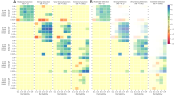
\includegraphics[width=1\textwidth]{figures/poly_panel_figure_2plots.pdf}
    \caption{Impact of Polygenicity on Populations' Survival. Panel \textbf{A} illustrates the effect of the number of contributing alleles (polygenicity) on populations' survival rates through the fitted logistic regression slopes between polygenicity and survivorship. Each colored square represents one slope/error value when all the reminaing parameters are kept constant as indicated in the figure, providing a comprehensive view of how polygenicity interplays with these factors. In panel \textbf{B} the survival rates of populations are superimposed with varying degrees of transparency, visually emphasizing areas of lower (less transparency) or higher mortality (more transparency). These plots highlight the critical importance of polygenicity, especially at the margins of survival, in shaping the evolutionary outcomes of populations.}
    \label{fig:poly_panel_figure}
\end{figure}

\begin{figure}[b]
    \centering
    \includegraphics[width=1\textwidth]{figures/meanfitness_varfitness_gen0to4.pdf}
    \caption{Mean Fitness and Fitness Variance at the Extinction Edge based on Genetic Architecture. Panel B depicts the mean fitness across two generations (Generation 0 and Generation 4) for varying levels of polygenicity, initial allele frequency range of contributing loci and heritability levels. Panel B illustrates the corresponding fitness variance for the same generations and genetic architectures. These results correspond to simulations with a fixed selection strength of Vs = 0.01 and whose new optimum was situated 2 standard deviations from the initial population phenotypic mean}
    \label{fig:meanfitness_varfitness_gen0to4}
\end{figure}

\begin{figure}[b]
    \centering
    \includegraphics[width=1\textwidth]{figures/mean_fitness_acrossgen.pdf}
    \caption{Evolution of Mean Fitness at the Extinction Edge based on Genetic Architecture. Changes in mean fitness across generation for different initial allele frequency and polygenicity of contributing loci and heritabilty levels. These results correspond to simulations with a fixed selection strength of Vs = 0.01 and whose new optimum was situated 2 standard deviations from the initial population phenotypic mean.}
    \label{fig:mean_fitness_acrossgen}
\end{figure}

\begin{figure}[b]
    \centering
    \includegraphics[width=1\textwidth]{figures/var_fitness_across_gen.pdf}
    \caption{Evolution of Fitness Variance at the Extinction Edge based on Genetic Architecture. Changes in fitness varince across generation for different initial allele frequency and polygenicity of contributing loci and heritabilty levels. These results correspond to simulations with a fixed selection strength of Vs = 0.01 and whose new optimum was situated 2 standard deviations from the initial population phenotypic mean.}
    \label{fig:var_fitness_across_gen}
\end{figure}

\begin{figure}[b]
    \centering
    \includegraphics[width=1\textwidth]{figures/metrics_boxplots-1.pdf}
    \caption{Caption of the figure.}
    \label{fig:metrics_boxplots}
\end{figure}

\begin{figure}[b]
    \centering
    \includegraphics[width=1\textwidth]{figures/metrics.pdf}
    \caption{Caption of the figure.}
    \label{fig:metrics}
\end{figure}


%% Supplementary figures 

\begin{figure}[b]
    \centering
    \includegraphics[width=1\textwidth]{figures/survivorshipforh2-1.pdf}
    \caption{Populations' survivorship across different values of polygenicity, initial allele frequency of contributing loci, strength of selection regimens and distance to new optimum.}
    \label{fig:survivorshipforh2}
\end{figure}

\begin{figure}[b]
    \centering
    \includegraphics[width=1\textwidth]{figures/survivorship_forpoly-1.pdf}
    \caption{Populations' survivorship across different values of heritability, initial allele frequency of contributing loci, strength of selection regimens and distance to new optimum.}
    \label{fig:survivorship_forpoly}
\end{figure}

\setcounter{figure}{0}
\renewcommand{\thefigure}{S\arabic{figure}}
\begin{figure}[b]
    \centering
    \includegraphics[width=1\textwidth]{figures/phenotypes_initial-3.pdf}
    \caption{Initial Phenotype Distributions Across Genetic Architectures. This figure presents the initial phenotypic distributions for populations with different levels of polygenicity, initial allelefrequency and heritability. Each plot shows the Kernel Density Estimate (KDE) of phenotypic values.}
    \label{fig:phenotypes_initial}
\end{figure}

\begin{figure}[b]
    \centering
    \includegraphics[width=1\textwidth]{figures/phenotypes_initial_onlymonogenic-2.pdf}
    \caption{ Initial Phenotype Distribution in Monogenic Architectures. This figure depicts the distribution of initial phenotypic values in populations where only one allele contributed to the trait value and varying initial allele frequency ranges and heritability values. The distribution is shown as a Kernel Density Estimate (KDE) of phenotypic values. This visualization highlights effect of heritability on low complecity architectures, where high heritability values normalize the phenotypes distributions.}
    \label{fig:phenotypes_initial_mono}
\end{figure}

\begin{figure}[b]
    \centering
    \includegraphics[width=1\textwidth]{figures/genetic_values_vs_lowheritability_difpoly.pdf}
    \caption{Comparative Analysis of Phenotype Distributions Across Various Polygenicity Levels Under Antagonistic Heritability Levels. Panel A illustrates the phenotypes' frecuency assuming a heritability of 1 for all combinations of polygenicity and initial allele frequency range for the trait contributing loci. Panel B presents the same range of polygenicity and initial allele frequency levels for the contributing loci but with a significantly reduced heritability of 0.1.}
    \label{fig:genetic_values_vs_lowheritability_difpoly}
\end{figure}


\section{Discussion}

\subsection{How to determine rapid evolutionary outcomes?}

With environments changing faster than ever, understanding the evolutionary dynamics of rapid adaptation has become of utmost interests. Application of this knowledge range from  invasive species management (Lee 2002; Lee and Gelembiuk 2008), applied evolutionary rescue for species at extinction risk, or even understanding  concerning medical issues such as the emergence of novel infectious diseases where genetic adaptation to a novel host is required (Holt and Hochberg 2002; Antia et al. 2003).

Rapid adaptation has been widely documented as shown in the examples listed in the introduction. Nonetheless, this does not mean that it can always occur. The mentioned examples highlight the \textbf{potential}, in principle, for rapid adaptation to overcome environmental changes. However, the large number of species that are becoming extinct, not only due to habitat transformations or hunting but also climate change, provide a tangible evidence that adaptation to rapid environmental changes is not a given (cite extinction list IPBES). Decades ago, theoretical work with simplified population genetic models \citep{Gomulkiewicz1995-sj} concluded that regardless of the genetic model, even populations with the necessary genetic variation to adapt, may still often fail to do so in novel environments. We therefore need to better understand when evolutionary outcomes will fail, and for that we need better understanding on key evolutionary and population parameters in realistic simulations and experiments. For example, it is now widely regarded that the  probability  of  a population  survival  increases  nearly  linearly  with  both  population  size  and  the number of exchangeable loci (diversity) (cite). Perhaps by identifying measurable parameters describing the genetics of a species, we may be able to improve practical management decisions for species conservation. 

\subsection{Genetic architecture is a key parameter defining evolutionary outcomes}

The literature on the relationship between rapid evolutionary outcomes and genetic architecture is inconclusive. In this study I thus focus on key parameters of an adaptive trait genetic architecture: number and initial frequency of contributing loci and heritability, under a gradient of selective pressures. 

Some foundational work on this topic was conducted by Gomulkiewicz \& Holt, who originally examined a quantitative-genetic model and a one-locus model  and obtained qualitatively similar results in terms of evolutionary outcomes \citep{Gomulkiewicz1995-sj}.  Furthermore, most studies from a decade ago, according to the 'selective sweep paradigm'  have focus on the dynamics of a trait determined by a single locus that is sufficient to rescue a population exposed to an environmental shift (Hermisson and Pennings 2005;  Hermisson and Pennings 2005; Barrett and Schluter 2008). Later on, Orr and Unckless, already highlighted the fact that it would be difficult for a single locus to adapt to rapid environmental change compared with the case for multiple loci where any one of them can rescue the population \citep{Orr2014-yn}, a concept now refered as genetic redundancy (cite yeaman). Later on,  in a theoretical work, Gomulkiewicz showed that increasing the number of loci can decrease the speed of adaptation and prevent the resultant rescue from extinction \citep{Gomulkiewicz2010-wr}. These results appear to contradict ours, and thus we explore the assumptions and differences of their models further. 

The contrasting difference between their and our approach is the definition used for fitness. They use an additive model of Malthusian fitness at time $t$ 
\[
m_t = \sum_{i=1}^{n} \left( p_{t,i}^2 m_{AA,i} + 2p_{t,i} q_{t,i} m_{Aa,i} + q_{t,i}^2 m_{aa,i} \right)
\]
where  
$n = \text{Number of loci}$, $p_{t,i} = \text{Frequency of allele A at locus } i \text{ at time } t$, 
$q_{t,i} = \text{Frequency of allele a at locus } i \text{ at time } t$, $m_{AA,i} = \text{Fitness of the AA genotype at locus } i$,
$m_{Aa,i} = \text{Fitness of the Aa genotype at locus } i$,
$m_{aa,i} = \text{Fitness of the aa genotype at locus } i $. They define $A$ as the advantageous allele at the new environment, and hence selection acts on the other two genotypes, so $m_{AA,i} = \frac{r_{\text{max}}}{n}$, $\text{ } m_{Aa,i} = \frac{r_{\text{max}}}{n - \frac{s_i}{2}} $, and $m_{aa,i} = \frac{r_{\text{max}}}{n - s_i} $
Where $r_{\text{max}}$ represent the maximum population growth and $s$ the selection coefficient. 
From this initial equation, they assume initial fitness mean and variance are constant across architectures to then derive populations' mean growth throughout generations for different polygenicity levels. Their results show an inverse relationship between the number of loci involved in the adaptation, and the population growth rate, since larger $n$ weaken the selection at each locus. But given their assumption of constant fitness mean and variance across genetic architectures, it is clear from their additive model, that selective pressure would be diluted when $n$ increases, which we argue, since selection acts on traits, not on loci. 

Oppositely, in our approach, fitness is a function of phenotypic values, and the same phenotype can be achieved with multiple genetic architectures. Furthermore, different genetic architectures lead to different initial mean fitness and variance.  \ref{fig:mean_fitness_acrossgen}, \ref{fig:var_fitness_across_gen},  \ref{fig:meanfitness_varfitness_gen0to4}. We observe even more variation for high heritability levels (they assume heritability to be 1 throughout their model). 

<<I think much of the behaviour may be explained too by the lack of finite populations in their models>>

Finally, our results are in concordance with more recent work by, Kardos \& Luikart  \citep{Kardos2021-jd}. In their study,  they use simulations to develop more realistic scenarios and demonstrated that population extinction is less likely in models with polygenic architectures compared with models with few large-effect loci due to their lower short-term evolutionary potential.

\subsection{Why does polygenicity increases the odds of survival at the extinction edge?}

<<I think this should be moved together with the upper one>>

Based on our observation, increased trait polygenicity has a positive effect on the survivorship probability at the extinction edges (\ref{fig:poly_panel_figure}), and independently of initial mean and variance fitness, more polygenic traits reach higher mean  and variance fitness after only 10 generations (\ref{fig:mean_fitness_acrossgen},  \ref{fig:var_fitness_across_gen}, \ref{fig:meanfitness_varfitness_gen0to4}). We argue that this results are based on two main things: 
\begin{enumerate}
    \item Polygenic architectures can generate exponentially more phenotypes, distributed in a more continuous manner. In polygenic architectures, the effect of each loci starts to be tiny on the overall phenotype, and the combinatorics of all loci creates a continuous distribution of phenotypes \ref{fig:genetic_values_vs_lowheritability_difpoly}. The opposite is true for low polygenic architectures. Low polygenic architectures can produce a lower number of resultant phenotypes, and their distribution is highly dependent on the initial allele frequency of the contributing loci (\ref{fig:genetic_values_vs_lowheritability_difpoly}). This tight link between low polygenic architectures and initial allele frequency of contributing loci, end up in more disruptive distribution of phenotype. Overall, the chances of phenotypes produces by low polygenic architectures to be adaptive are not constant. 

    \item Redundancy: One central property of the genetic architecture of polygenic traits is the general many-to-one relationship, a single phenotype corresponds to a larger number of genotypes. These genotypes are thus redundant with respect to the phenotype they produce and individuals can use different sets of alleles to generate the optimal phenotype. This has been already hihgligted by \citep{Orr2008-jl}. 
\end{enumerate}

\subsection{High heritability does not improve survival in low complexity traits}

Our results show that at low polygenic architectures, heritability does not increase the chances of survivorship. Opposite to that, depending on the initial allele frequency of the contributing loci, heritability might correlate negatively with survivorship. (\ref{fig:h2_panel_figure}).

Heritability is known as evolution's memory.  Selection operates on heritable traits, and for a trait to evolve through selection, it must be at least partly heritable. If a trait that provides an advantage is heritable, it is more likely to be passed on to the next generation.  In this sense, our results are contraintuitive. Nevertheless, under high heritability (when the phenotype is mainly determined by the genetic value) low complexity architectures are very susceptible to the initial frequency and showcase more stochastic distributions of phenotypes, as explained in the previous section. On the other hand, low heritability, acts as a normalization force of discrete phenotypes. Filling in the gaps, low heritability gives low polygenic architectures, just by chance, a higher probability of survivorship.

I think this section and the results of h2 may need to be better connected with the conondrum from the previous section, and ask what is the relationship of h2 (Va/Vtotal) and Va. 
Is this a demographic argument? that allows you not to completely lose the population even if you have low Va and thus low adaptive potential?

\subsection{Polygenicity is not intrinsically better}

As stated by Lande, early on 1983, adaptation from polygenic or monogenic traits is equally feasible  \citep{Lande1983-kz}, and we believe so, under the assumption that they can both achieve the optimum trait value. We believe that, if the trait value is adaptive, independent of its genetic architecture it will have enough fitness to rescue the population from extinction. Nevertheless, higher polygenic architecture will cover the phenotypic space in a more continuous and consistent manner, enhancing their odds to adaptation to further optima. 

We would like to highlight the fact that our results are true under two main assumptions: the new optimum is on a reachable range and adaptation is solely based on standing variation. This is quite important, since in an scenario where the new optimum value is out of range and standing genetic variation wouldn't be enough to reach it, the opposite might be true. If the optimum is far enough, so all current population phenotypes would have a fitness of 0 in the new environment, escaping extinction would only rely on \textit{de novo} mutations. In this case, the number of mutations needed for a trait to adapt to a new far optimum, would be less in the case of the low complexity architecture, while in the case of highly polygenic architecture, many mutations would be needed, to coordinate a new trait value. Based on this, we highlight that our results would be more applicable in a context of environmental shift that do not exceed a magnitude where the population's genetics would be completely maladaptive. For example, this wouldn't be applicable to invasive species where the population might be entirely unsuited to the new environment. 

We conclude that, if the genetic variance exist for adaptation to the new optimum, polygenic architectures show more robust adaptive capacity reaching further new optimum. Low polygenic architectures, might or might not adapt and are higly dependent on initial allele frequency of contributing loci. Overall, low polygenic architecture do not produce 'worst' phenotypes they just produce less and disruptive distributed phenotypes. 

\subsection{Novel GWA across environments are needed to identify causal adaptive loci to different climates}
<<after reading all of it, it looks more and more like this section may not fit into the narrative. I suggest remove, but we can discuss about this. I think unless this section is developed much more it looks like it misses a leg>>
Our results show that current available tools are not yet suited for the identification of adaptive loci in the context of an E\&R experiment across environemnts in an an organisms with high self fertilization rates. 
The lack of recombination will lead to the formation genetic blocks are during polygenic selection under self fertilisation \citep{Hartfield2022-nc}. Adaptive loci will increse in frequency, but will take with them a block of neutral hitchickers. This is particularly complicates the identification of adaptive loci. 

Nonetheless we believe that this problems can be overcome with the developing of new statistical approaches. 

\subsubsection{Final comments}
Our model is subjective, and it lives under simplifying  assumptions, while also igorning other biologically relevant parameters. But we also believe that the simplicy allows to hihglight key interactions. We did not model different demographic scenarios, nor population sixes, we didn't explore further in a two trait models to include higher level interactions like epistasis, or pleiotropy. 

We also know that teh cost of using real genetic data from A. thaliana, makes oru results subscriptive to a population with low outcrossing rates, and hence low recombinations rates. Also, because A. thalina  reproductive excess may be able to accommodate high levels of mortality without a decrease in adult population size if growth rate is not reduced to below replacement (Crow 1970, paper from moi).


On this set of simulations we have inspired ourselves on the experimental set up of GrENE-NET and on the biology of A. thaliana. 
Polygenic selection has been extensively studied in models assuming random–mating. Yet many species self fertilise to some degree, which incurs changes to genetic diversity, recombi- nation and genome segregation. Studying selfing might be of paritucalr importance in agricultural relvant crops. Even though, low complexity or hihgly polygenic architecutres haven described in mixed mating organissm like Mimulus  guttatus;  Troth et  al. (2018) but also in hihgly selfing selfing plant Arabidopsis  thaliana (Zan  and  Carlborg  2018;  Exposito-Alonso et  al. 2018;  Tsuchimatsu et al. 2020; Wieters et al. 2021), but studies of genetic architecture implication of the evolutionary outcome have only been described in models assuming random–mating, and we could ppnly find one work where the evolutionary outcomes of selfing was explored \citep{Hartfield2022-nc}.




\subsection{to do}
- create figure for var in fitness to cite
- make sure all figures abor fitenss variance and fitness mean are about the same little square 

\subsection{extra}
explore if in the polygenic or monogenic adaptation the alleles of high or low effect persisted

I should calcualte the 'selection limits' bascialyl the difference between mean phenotypes at gen 4 - mean pheno gen 0 
Calculation of L0: L0 is calculated as the difference between the predicted mean phenotype at ten generations and the mean phenotype at the beginning of the simulation.
Regression Analysis: A regression analysis is used to measure the relationship between L0 and population viability. Specifically, generalized linear models (GLMs) with a logit link function in R are used, with population persistence as the response variable, coded as 0 for extinct populations and 1 for populations that persisted

compare the r squared of the casual with the one from the non causal

% backlog 


\bibliography{paperpile} % Bibliography

\end{document}
